\documentclass{article}
\usepackage{amsmath, amssymb, amsthm, amsfonts, bm}
\theoremstyle{remark}
\newtheorem*{theorem}{Theorem}
\newtheorem*{remark}{Remark}
\newtheorem*{definition}{Definition}
\newtheorem*{hypothesis}{Hypothesis}
\newtheorem*{corollary}{Corollary}
\theoremstyle{remark}

\usepackage{physics}
\usepackage[a4paper, total={6in,10in}]{geometry}
\usepackage[dvipsnames]{xcolor}
\usepackage{xcolor-material}
\usepackage{hyperref}
    \hypersetup{colorlinks=true, linkcolor=ForestGreen}
\usepackage{graphicx}
    \graphicspath{{./img/}}
\usepackage{tikz}
\usepackage{ragged2e}
\usepackage{array}   % for \newcolumntype macro
\newcolumntype{L}{>{$}c<{$}} % math-mode version of "l" column type

\usepackage{soul}

\newcommand{\where}[1]{\begin{flushright}where #1.\end{flushright}}
\newcommand{\wher}[1]{\begin{flushright}#1.\end{flushright}}
\newcommand{\mylabel}[2]{\hyperref[#1]{#2}\label{back:#1}}
\newcommand{\myref}[1]{\hyperref[back:#1]{$\bigstar$}\label{#1}}
\newcommand{\e}{\hat{\vb{e}}}  % unit vector
\newcommand{\s}[1]{\textsubscript{#1}}
\everymath{\displaystyle}
\begin{document}

\begin{enumerate}
    \item $\boxed{r=\frac{r_0}{1+e\cos\phi}}$
    \item $\boxed{J^2 = Amr_0}$
    \item Has a different origin to $\frac{x^2}{a^2}+\frac{y^2}{b^2}=1$, $\frac{x^2}{a^2}-\frac{y^2}{b^2}=1$ but same shape
    \item $r_{\mathrm{min}}=\frac{r_0}{1+e}$, $r_{\mathrm{max}}=\frac{r_0}{1-e}$
    \item $F=-\frac{A}{r^2}$
    \item Kepler\begin{itemize}
        \item 1st Trajectory are ellipses
        \item 2nd $\dv{\mathrm{Area}}{t}=r^2\dot\phi/2=\frac{J}{2m}$ is constant
        \item 3rd $T^2 \propto a^3$ (Rearrange polar to cartesian, semi-major $a=\frac{r_0}{1-e^2}$, semi-minor $b=\frac{r_0}{\sqrt{1-e^2}}$, $T=\frac{\pi ab}{\mathrm{area\ change\ rate}}=2\pi\sqrt{\frac{ma^3}{A}}$)
    \end{itemize}
    \item A cool thing I wasn't aware of is that $\dv{t}(r^2) = 2r\dv{r}{t} = \dv{t}(\vec{r}\cdot\vec{r}) = 2\vec{r}\cdot\dv{\vec{r}}{t}$, which is not immediately obvious
    
    $\dv{r}{t} = \hat{r}\cdot\dv{\vec{r}}{t}$ (draw a picture)

    \item $\vb{J}=\sum\vb{r}\times\vb{p}=\sum\vb{r}\times m(\bm{\omega}\times\vb{r})=\textcolor{red}{\sum m(r^2\bm{\omega}-\vb{r}(\vb{r}\cdot\bm{\omega}))} = \sum m(\bm{r}^T\bm{r}\bm{1}-\bm{r}\bm{r}^T)\bm{\omega} = \bm{I}\bm{\omega} = \begin{pmatrix}
        \textstyle\sum m(y^2+z^2) & -\textstyle\sum mxy & -\textstyle\sum mxz\\
        -\textstyle\sum mxy & \textstyle\sum m(x^2+z^2) & -\textstyle\sum myz\\
        -\textstyle\sum mxz & -\textstyle\sum myz & \textstyle\sum m(x^2+y^2)\\
    \end{pmatrix}\bm{\omega} $

    ($I$ is Hermitian, principle axes orthogonal)

    \item $T = \frac{1}{2}\sum m(\bm{\omega}\times\bm{r})\cdot(\bm{\omega}\times\bm{r}) = \frac{1}{2}\sum m\bm{\omega}\cdot(\bm{r}\times(\bm{\omega}\times\bm{r})) = \frac{1}{2}\bm{\omega}\cdot\bm{J} = \frac{1}{2}\bm{\omega}^T I\bm{\omega}$
    
    The surface of constant $T$ is a quadric surface called Inertia Ellipsoid. $\grad_{\bm{\omega}}T=\bm{J}$, $\bm{J}$ is perpendicular to the surface of constant $T$

    \item Perpendicular axes theorem for sheets, parallel axes theorem $I=I_0+Ma^2$ for $I_0$ at CoM at $\bm{a}$ from the origin
    \item Kater's pendulum, parallel axes theorem + pendulum = determine $g$ by measuring small oscillation period $T$ and $a$
    \item For body frame $S$, $\bm{G}=\left[\dv{\bm{J}}{t}\right]_S+\bm{\omega}\times\bm{J}$, Euler's equations are \begin{align*}
        G_1 = I_1\dot\omega_1 + (I_3-I_2)\omega_2\omega_3\\
        G_2 = I_2\dot\omega_2 + (I_1-I_3)\omega_3\omega_1\\
        G_3 = I_3\dot\omega_3 + (I_2-I_1)\omega_1\omega_2
    \end{align*}
    
    (Because $\bm{J}=I\bm{\omega} = \sum_{i=1}^{3} I_i\omega_i\hat{e}_i$, $\bm{G}=\sum_{i=1}^{3} I_i\dot\omega_i\hat{e}_i+I_i\omega_i\dv{\hat{e}_i}{t}$ and $\boxed{\dv{\hat{e}_i}{t}=\bm{\omega}\times\hat{e}_i}$)
    \item For a symmetric top ($I_1=I_2\neq I_3$), body freqency $\boxed{\Omega_b\equiv\frac{I_1-I_3}{I_1}\omega_3}$\begin{itemize}
        \item In the body frame $S$, $\bm{J}$ and $\bm{\omega}$ in the same plane because $I_1=I_2$, and if oblate inertia ellipsoid (prolate top), $I_3>I_2$, $J_3=I_3\omega_3>I_1\omega_3$, $\bm{J}$ inside the cone of $\bm{\omega}$
        \begin{center}
            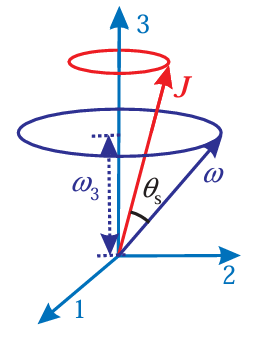
\includegraphics[width=0.25\linewidth]{symmetric top body frame.png}
        \end{center}
        \item In the inertial frame $S_0$, rate of precession $\boxed{\Omega_s=\frac{\dot\omega_1}{|\bm{\omega}|\sin\theta_s}=\frac{J}{I_1}}$
        \begin{center}
            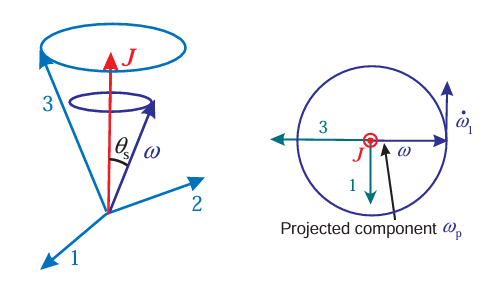
\includegraphics[width=0.6\linewidth]{rate of precession.png}
        \end{center}
        \item Ellipsoid tangential to invariable plane ($\grad_{\bm{\omega}}T=\bm{J}$), and rolls without slipping on it. 
        \[\boxed{\Omega_b\sin\theta_b=\Omega_s\sin\theta_s}\]
        \begin{center}
            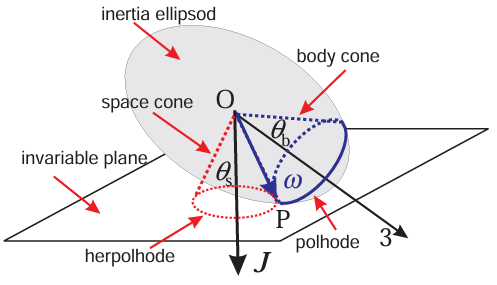
\includegraphics[width=0.6\linewidth]{poinsot.png}
        \end{center}
    \end{itemize}
    \item For triaxial body with $I_1<I_2<I_3$, if the body spins about the 2-axis is unstable. $\bm{\omega}$ can change while keeping $\bm{J}$ and energy constant.
    \item Major axis theorem: non-rigid bodies will align their $\bm{J}$ to the major axis to minimize energy
    \item Symmetric top with Euler angles $(\theta,\phi,\chi)$
    
    \begin{minipage}[b]{0.6\textwidth}
        \centering
        \begin{itemize}
            \item $\bm{\omega}=\dot\phi\hat{e}_z+\dot\theta\hat{e}_1+\dot\chi\hat{e}_3$
            \item In body frame $S$, $\bm{\omega}=(\dot\theta,\dot\phi\sin\theta,\dot\chi+\dot\phi\cos\theta)$
            
            $\bm{J}=(I_1\dot\theta,I_1\dot\phi\sin\theta,I_3(\dot\chi+\dot\phi\cos\theta))$
            \item Keep $\omega_3=\dot\chi+\dot\phi\cos\theta$, $J_z=J_3\cos\theta+J_2\sin\theta$ constant
            \item We get $\dot\phi=\Omega_s$, $\dot\chi=\Omega_b$
        \end{itemize}
    \end{minipage}
    \hfill
    \begin{minipage}[b]{0.39\textwidth}
        \centering
        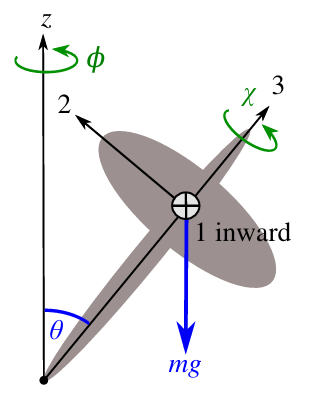
\includegraphics[width=0.4\linewidth]{Lagrange's approach.png}
    \end{minipage}

    \item Equation of motion with gravity and support
    \begin{align*}
        E &= \frac{1}{2}I_1\omega_1^2 + \frac{1}{2}I_1\omega_2^2 + \frac{1}{2}I_3\omega_3^2+mgh\cos\theta\\
          &= \frac{1}{2}I_1\dot\theta^2 + \frac{J_2^2}{2I_1} + \frac{J_3^2}{2I_3}+mgh\cos\theta\\
          &= \frac{1}{2}I_1\dot\theta^2 + \frac{(J_z-J_3\cos\theta)^2}{2I_1\sin^2\theta} + \frac{J_3^2}{2I_3}+mgh\cos\theta\\
          &= \frac{1}{2}I_1\dot\theta^2 + U_{\mathrm{eff}}(\theta)
    \end{align*}

    \item Sleeping top $J_z=J_3$; if $\dv{U_{\mathrm{eff}}}{\theta}=0$ steady precession; oscillation around $\theta$ is nutation
    \begin{center}
        \includegraphics*[width=0.3\linewidth]{symmetric top effective potential.png}
    \end{center}

    \item $\mathcal{L}=T-V$, $\dv{t}\pdv{\mathcal{L}}{\dot q_i}=\pdv{\mathcal{L}}{q_i}$
    \item Conjugate momenta $p_i=\pdv{L}{\dot q}$, symmetry (\textbf{invariance} of $\mathcal{L}$ wrt. $q_i$ leads to \textbf{conservation} of $p_i$)
    \item Hamiltonian $H(q_i,p_i,t)\equiv\sum_i p_i\dot q_i-\mathcal{L}(q_i,\dot q_i,t)$, 
    $\dd H=\sum_i\left(\dot q_i\dd p_i-\dot p_i\dd q_i\right)-\pdv{\mathcal{L}}{t}\dd t \allowbreak= \sum_i\left(\pdv{H}{q_i}\dd q_i+\pdv{H}{p_i}\dd p_i\right)+\pdv{H}{t}\dd t \allowbreak= -\pdv{\mathcal{L}}{t}$ (depends only on $q_i,p_i,t$, not $\dot q_i$)
    \item $\pdv{H}{t}=-\pdv{\mathcal{L}}{t}$ means if $\mathcal{L}$ is independent of $t$, then energy/Hamiltonian is conserved
    \item $\dot q_i=\pdv{H}{p_i}$, $\dot p_i=-\pdv{H}{q_i}$
    \item $\epsilon=x-x_0$, $m\ddot x+\dv{U}{x}=0$, $m\ddot\epsilon+U_0''\epsilon=0$
    \item In a \textbf{normal mode} every element of the system oscillates at a single frequency, a general free oscillation of the system can be expressed in terms of a linear combination of the single normal modes.
    \item $\vb{r}=\vb{r}(\{q_i\})$, around equilibrium $\bm{\dot r}\approx\sum_i\dot q_i\eval{\pdv{\bm{r}}{q_i}}_{\mathrm{eq}}$, $T=\frac{1}{2}\sum_k m_k|\bm{\dot r}_k|^2 = \frac{1}{2}\sum_{ij}M_{ij}\dot q_i\dot q_j = \frac{1}{2}\bm{\dot q}^T\bf{M}\bf{\dot q}$, $M_{ij}=\sum_k m_k\eval{\pdv{\bf{r_k}}{q_i}}_{\mathrm{eq}}\eval{\pdv{\bf{r_k}}{q_j}}_{\mathrm{eq}}$
    \item At equilibrium $\eval{\pdv{U}{q_i}}_{\mathrm{eq}}$, $U=U(\bm{q})\approx U_0+0+\frac{1}{2}\sum_{ij}q_i q_j\eval{\pdv{^2U}{q_i \partial q_j}}_{\mathrm{eq}}+\ldots$, $K_{ij}=\eval{\pdv{^2U}{q_i \partial q_j}}_{\mathrm{eq}}$
    \item At equilibrium $E\approx U_0+\frac{1}{2}\sum_{ij}M_{ij}\dot q_i\dot q_j+\frac{1}{2}\sum_{ij}K_{ij}q_i q_j$, $\dv{E}{t}=0=\sum_{ij}\dot q_i(M_{ij}\ddot q_j+K_{ij}q_j)$, $\boxed{\bm{M}\vb{\ddot q}+\bm{K}\vb{q}=0}$, together with guessed solution $\boxed{\vb{q}(t)=\vb{Q}e^{i\omega t}}$, $(\bm{K}-\omega^2\bm{M})q = 0$
    \item $\bm{M}$ and $\bm{K}$ are symmetric, thus $\omega_i$ are real
    \item \begin{itemize}
        \item $(\vb{K}-\omega^2 \vb{M})\vb{q}=0$, $\vb{K},\vb{M}$ are symmetric, $\omega^2$ is real
        \item $(\vb{M}^{-1}\vb{K}-\omega^2\vb{I})\vb{q}=0$, $\vb{M}^{-1}\vb{K}$ not symmetric in general, $\vb{q}_i\cdot\vb{q}_j\neq0$ in general (product of symmetric matrices may not be symmetric)
        \item $(\vb{M}^{-1/2}\vb{K}\vb{M}^{-1/2}-\omega^2\vb{I})(\vb{M}^{1/2}\vb{q})=0$, inverse and square root of symmetric matrices are symmetric, $\vb{M}^{-1/2}\vb{K}\vb{M}^{-1/2}$ is symmtric, $\boxed{\vb{q}_i^T\vb{M}\vb{q}_j = \delta_{ij}}$
        \item To find orthonormal modes, turn $\vb{M}$ into $\vb{I}$ and normalize $\vb{q}$
    \end{itemize}
    \item Young's modulus $E=\frac{P}{\delta l/l}$, Bulk modulus $B=-\frac{P}{\delta V/V}$ ($\Delta V<0$)
    \item $\dd\vb{F}=\bm{\tau}\dd\vb{S}=A\bm{\tau}\cdot\hat{\vb{n}}$, the stress tensor is $\bm{\tau}=\begin{pmatrix}
        \tau_{xx} & \tau_{xy} & \tau_{xz} \\
        \tau_{yx} & \tau_{yy} & \tau_{yz} \\
        \tau_{zx} & \tau_{zy} & \tau_{zz}
    \end{pmatrix}$, $\tau_{xx}$ is normal stress, $\tau_{xy}$ is shear stress
    \item $\vb{X}=\vb{e}\vb{x}$, the strain tensor is $\vb{e}=\begin{pmatrix}
        e_{xx} & e_{xy} & e_{xz}\\
        e_{yx} & e_{yy} & e_{yz}\\
        e_{zx} & e_{zy} & e_{zz}\\
    \end{pmatrix}$ is symmetric, $\boxed{e_{ij}=\frac{1}{2}\left(\pdv{X_i}{x_j}+\pdv{X_j}{x_i}\right)}$, can be diagonalized to $\vb{e}=\begin{pmatrix}
        e_1 & 0&0\\
        0 & e_2&0\\
        0 & 0&e_3\\
    \end{pmatrix}$
    \item For simplicity, only consider principal axis to express $e$ and $\tau$ as vectors
    \item Strain is $e=\delta l/l$, stress is $\tau=-P=-F/A$, for isotropic material, $\textstyle E\vb{e}=\begin{pmatrix}
        1 & -\sigma & -\sigma\\
        -\sigma & 1 & -\sigma\\
        -\sigma & -\sigma & 1
    \end{pmatrix}\bm{\tau}$, $\sigma$ is Poisson ratio, $e_1=e_2=e_3=\frac{\tau(1-2\sigma)}{E}$, $\frac{\delta V}{V}\approx e_1+e_2+e_3 = \frac{3\tau(1-2\sigma)}{E}$, $\boxed{B=\frac{E}{3(1-2\sigma)}}$
    \item $\bm{\tau}=\begin{pmatrix}
        1 & -\sigma & -\sigma\\-\sigma & 1 & -\sigma\\-\sigma & -\sigma & 1\end{pmatrix}^{-1}
        E\vb{e} = \frac{E}{(\sigma+1)(1-2\sigma)}\begin{pmatrix}
            1-\sigma & \sigma & \sigma\\
            \sigma & 1-\sigma & \sigma\\
            \sigma & \sigma & 1-\sigma\\
        \end{pmatrix}\vb{e} = \lambda(e_1+e_2+e_3)+2G\bm{e} = \lambda\Tr(\bm{e})\bm{I}+2G\bm{e}$, Lam\'e's constant $\boxed{\lambda\equiv\frac{E\sigma}{(1+\sigma)(1-2\sigma)}, G=\frac{E}{2(1+\sigma)}}$, $\lambda=B-\frac{2}{3}G$
    \item The elastic potential energy of a small volume $(\Delta x,\Delta y,\Delta z)$ is \begin{align*}
        U &=\frac{1}{2}\Delta x\Delta y\Delta z(\tau_1 e_1+\tau_2 e_2+\tau_3 e_3) \\
        &= \frac{1}{2}\Delta x\Delta y\Delta z\left[\lambda(e_1+e_2+e_3)^2+2G(e_1^2+e_2^2+e_3^2)\right] \\
        &= \frac{1}{2}\Delta x\Delta y\Delta z\Tr(\bm{\tau}\bm{e})\\ 
        &= \frac{1}{2}\Delta x\Delta y\Delta z(\tau_{xx}e_{xx}+\tau_{yy}e_{yy}+\tau_{zz}+e_{zz}+2\tau_{xy}e_{xy}+2\tau_{yz}e_{yz}+2\tau_{xz}e_{xz})\\
        &= \frac{1}{2}\Delta x\Delta y\Delta z(\Tr[(\lambda \Tr(\bm{e})+2G\bm{e})\bm{e}])\\
        &= \frac{1}{2}\Delta x\Delta y\Delta z(\Tr(\bm{e})\Tr[\lambda\bm{e}]+2G\Tr[\bm{e}^2])\\
        &= \textcolor{red}{\frac{1}{2}}\Delta x\Delta y\Delta z\ (\textcolor{red}{\lambda[\Tr(\bm{e})]^2+2G\Tr(\bm{e}^2)})
    \end{align*}
    \item For a bending beam, the bending moment (sum of moment caused by all forces at cross section) is $\boxed{B=\frac{EI}{R}}$, moment of area $\boxed{I=\int_{\text{cross section}} y^2\dd A}$\begin{align*}
        B&=\int y\cdot\text{stress}\dd A \\
         &=\int yE\cdot\text{strain}\dd A \\
         &=\int yE\cdot\frac{\Delta l}{l}\dd A\\
         &=\int yE\cdot\frac{\theta(R+y)-\theta R}{\theta R}\dd A\\
         &=\int yE\frac{y}{R}\dd A
    \end{align*}
    where radius of curvature $R\approx \frac{1}{y''}$, $\boxed{B=EIy''}$
    \item For a general beam with load per unit length $W(x)$, $W=-\dv{F}{x},\boxed{F=-\dv{B}{x}}$, $\boxed{W=EIy''''}$
    \item Finding out bending moment: the beam is at equilibrium, so the part to the left of $x$ is at equilibrium, the RHS tip of this part --- element at $x$, is balanced by its bending moment and all the forces on the left (for non-rigid/elastic body, balance of force is a necessary insufficient condition of equilibrium)
    
    Interestingly, using this analysis, a beam freely supported at one end only cannot be in equilibrium, as the part to the right of the load cannot have $B(x)=0$. It must be clamped on the left to provide a torque so the $B(x)$ is moved upwards to make that 0.
    \item $B=-Fy,y''+\frac{F}{EI}y=0, y=A\sin\sqrt{\frac{F}{EI}}x$, Euler force $F_E=\frac{\pi^2 EI}{L^2}$, of $F<F_E$ the beam is compressed, if $F\geq F_E$ the beam will bend suddenly. (Note that $L$ also changes)\begin{center}
        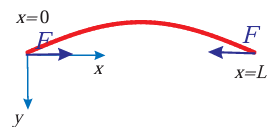
\includegraphics[width=0.24\linewidth]{euler_struct.png}
    \end{center}
    \item $\pdv{\rho}{t}+\div(\rho\vb{v}) = 0$, $\rho$ is a constant (incompressible), $\div\vb{v}=0$
    \item $\vb{v}(\vb{x},t)$, $\dd\vb{x}=\vb{v}\dd{t}$, convective/total derivative $\boxed{\frac{D\vb{v}}{D t}=\pdv{\vb{v}}{t}+\vb{v}\cdot\grad\vb{v}}$
    \item \textcolor{red}{Euler's equation} $\boxed{\rho\frac{D\vb{v}}{D t} = -\grad(P+\rho\phi_g) =-\grad P-\rho\grad\phi_g = -\grad P+\rho\vb{g}} $
    \item Streamlines, particle paths, streaklines
    \item Incompressible flow Bernoulli equation $\boxed{P+\frac{1}{2}\rho v^2+\rho\phi=C}$ along streamline
    \item Efflux coefficient is effective area/geometric area $<$ 1, Borda's mouthpiece 0.5
    \item Incompressible $\div\vb{v}=0$, irrotational vorticity $\vb{\omega\equiv\curl\vb{v}} = 0$, $\vb{v}=\grad\Phi$,$\laplacian\Phi=0$
    \item Circulation around a loop $\Gamma$ is $K=\oint_\Gamma\vb{v}\cdot\dd\vb{l}=\int_S(\curl\vb{v})\cdot\dd\vb{S}=\int\omega\cdot\dd\vb{S}$
    \item \begin{align*}\frac{D K}{D t}&=\oint_\Gamma\left(\frac{D\vb{v}}{D t}\cdot\dd\vb{l}+\vb{v}\cdot\frac{D(\dd\vb{l})}{Dt}\right) \\
                &= \oint_\Gamma\left(\grad(\frac{-P}{\rho}-\phi_g)\cdot\dd\vb{l}+\vb{v}\cdot\frac{D(\dd\vb{l})}{Dt}\right)\\
                &= \oint_\Gamma\left(\grad(\frac{-P}{\rho}-\phi_g)\cdot\dd\vb{l}+(\dd\vb{l}\cdot\grad)\vb{v}\right)\\
                &= \oint_\Gamma\left(\grad(\frac{-P}{\rho}-\phi_g)\cdot\dd\vb{l}+\grad(\frac{1}{2}v^2)\cdot\dd\vb{l}\right)\\
                &= \oint_\Gamma\grad\left(-\frac{P}{\rho}-\phi_g+\frac{1}{2}v^2\right)\dd\vb{l}\\
                &= 0
    \end{align*}because curl of gradient is 0
    \item $\boxed{\tau_{ij}=\eta\left(\pdv{v_i}{x_j}+\pdv{v_j}{x_i}\right)}=\eta\dv{2e_{ij}}{t}$ is the definition of viscosity $\eta$.
    \item Incompressible Navier-Stokes equation $\boxed{\rho\frac{D\vb{v}}{D t}=-\grad P+\rho\vb{g}+\eta\laplacian{\vb{v}}}$
    \item Poiseuille flow: steady state, $\frac{D\vb{v}}{Dt}=0$ ($\pdv{\vb{v}}[t]=0,\ \vb{v}\cdot\grad{\vb{v}}=0$), balance viscous shear force $\tau_{xy}\cdot\mathrm{area},\tau_{xy}=\eta\pdv{v_x}{y}$ ($v_y=0$ in these questions) and total force acted on this bulk of fluid (gravity/pressure difference ...), answer is parabolic velocity vs. distance
    \item Reynolds number $N_R=\frac{\rho v_0 d}{\eta}$ is a dimensionless number, where $\rho$ is density of fluid, $d$ is diameter of sphere/tube, $v_0$ is speed of sphere/average speed inside tube, $\eta$ is viscosity
    \item At high $N_R$ turbulence occurs. More viscous means lower $N_R$.
    \item Dipole (velocity) field (spherical BC): $\boxed{\Phi=v_0\cos\theta\left(r+\frac{a^3}{2r^2}\right)}$\begin{itemize}
            \item At \textcolor{red}{infinity, $\vb{v}=(v_0,0,0)$}, $\Phi=v_0x=v_0r\cos\theta$, $A_1=v_0$, $A_{i\neq 1}=0$
            \item $\Phi=\sum_{l=0}^\infty (A_l r^l+B_l r^{-l-1})P_l(\cos\theta)$
            \item At surface, $v_r=\dv{\Phi}{r}=0$, $v_0\cos\theta=\eval{(l+1)B_l r^{-l-2}P_l(\cos\theta)}_{r=a}$, $B_1=\frac{v_0a^3}{2}$
        \end{itemize}
\end{enumerate}

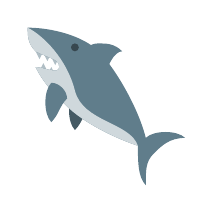
\begin{tikzpicture}
    \begin{scope}[scale=1/10]
    \fill [MaterialBlueGrey200] 
      (2,16.75) -- ++(0.5,-1) -- ++(0.5,1) -- cycle
      (3,16.25) -- ++(0.5,-1) -- ++(0.5,1) -- cycle
      (1,17)    -- ++(0.5,-1) -- ++(0.5,1) -- cycle
      (2,15.5)  -- ++(-.5,-1) -- ++(1,0) -- cycle
      (3,15)    -- ++(-.5,-1) -- ++(1,0) -- cycle;
    \fill [MaterialBlueGrey700] (6,12)
      .. controls (5,11) and (5,8)  .. (6,7)
      .. controls (7,8)  and (7,9)  .. (8,10)
      .. controls (8,11) and (7,12) .. (6,12)-- cycle;
    \fill [MaterialBlueGrey500] (0,20)
      .. controls (0,19)  and (0,18)  .. (1,17)
      .. controls (3,16)  and (4,16)  .. (4,15)
      .. controls (4,14)  and (2,15)  .. (1,15)
      .. controls (2,13)  and (3,12)  .. (5,10)
      .. controls (7,8)   and (11,6)  .. (14,5)
      .. controls (14,3)  and (14,1)  .. (15,0)
      .. controls (15,2)  and (15,3)  .. (16,4)
      .. controls (17,5)  and (18,6)  .. (20,6)
      .. controls (19,7)  and (16,7)  .. (15,6)
      .. controls (14,10) and (11,15) .. (9,17)
      .. controls (7,19)  and (3,20)  .. (0,20) -- cycle;
    \fill [MaterialBlueGrey100] (0,20)
      .. controls (0,19) and (0,18) .. (1,17)
      .. controls (3,16) and (4,16) .. (4,15)
      .. controls (4,14) and (2,15) .. (1,15)
      .. controls (2,13) and (3,12) .. (5,10)
      .. controls (7,8)  and (11,6) .. (14,5)
      .. controls (13,8) and (7,8)  .. (6,12)
      .. controls (5,16) and (2,19) .. (0,20) -- cycle;
    \fill [MaterialBlueGrey500] (3,13)
      .. controls (2,12) and (2,9)  .. (3,8)
      .. controls (4,9)  and (4,10) .. (5,11)
      .. controls (5,12) and (4,13) .. (3,13) -- cycle;
    \fill [MaterialBlueGrey500] (9,18)
      .. controls (8,18)  and (7.5,17.5) .. (7,17)
      .. controls (7,16)  and (9,14)     .. (10,14)
      .. controls (10,15) and (11,17)    .. (12,17)
      .. controls (11,18) and (10,18)    .. (9,18) -- cycle;
    \fill [MaterialBlueGrey800] (6,17.5) circle [radius=0.5];
    \end{scope}
    \end{tikzpicture}
    
\end{document}